\chapter{Evaluation}\label{evaluation}
This chapter starts by evaluating proposed neural network architectures using CPUs and GPUs to find a baseline inference latency, accuracy and AUC values. This information is then compared with the results obtained from simulating and synthesizing the models on reconfigurable hardware. The outcome of the design space exploration includes hardware resource utilization metrics as well as discussion about the Pareto front and applicability in high energy physics environments. Lastly, both the pre-training and post-training quantization are evaluated quantitatively in terms of the trade-off between quality of results and bit-width reduction as well as qualitatively for their ease of adaptation to existing designs.

% This chapter outlines the proposed evaluation plan for the project. The first objective of developing and optimizing a state-of-the-art neural network in hardware can be evaluated quantitatively, while integrating it into the \textit{hls4ml} library and making it easy for new users to use requires a more qualitative approach.

% \section{Quantitative results}
% The following describes the quantities to be measured for each neural network design:

% \begin{outline}
%   \1 Classification accuracy, AUC and confusion matrix on a validation dataset
%   \1 Inference latency and throughput when running on the target platform
%   \1 Hardware resource utilization (exact values for comparison with other platforms and percentage of available resources for understanding limitations):
%     \2 Block RAM (BRAM) and Ultra RAM (URAM)
%     \2 Digital Signal Processing units (DSP)
%     \2 Flip-Flops (FF)
%     \2 Look-Up Tables (LUT)
% \end{outline}

% In the early stages of the project, the above quantities will be measured from the results from the simulation and synthesis reports. At a later stage, the best designs will be run on actual hardware platforms to validate them under real-life use cases. The platform planned for this part is an Intel Stratix V FPGA hosted in a Maxeler MPC-X dataflow node with 8 Maia dataflow engines and 48 GB of DRAM. A consideration is also planned for the specific hardware used in the LHC L1T detectors and its available resources, which although cannot be directly tested on, can guide the state space exploration.

% Apart from clear design improvements, it is predicted that most evaluated designs will offer trade-offs between classification accuracy, AUC, inference throughput and hardware utilization. It is not possible to find a design that is superior in every way, hence a Pareto front and the Roofline model will play the key roles in understanding the overall performance and selecting configuration with specific needs in mind.


% \section{Qualitative Results}
% To assess the success of enhancing the \textit{hls4ml} library, qualitative comparisons will be drawn between it and the already existing neural network components and architectures. Depending on the project's timeline, it is possible that the improvements can get official approval and get merged into the main repository, however if this is not feasible before the final deadline, current users of the library will be surveyed and their opinion will be taken into consideration instead.

\section{Architecture Analysis}
\indo{Carries on from chapter 3}
\indo{|}
\indo{|}
\indo{|}

\subsection{Existing Solutions}

\begin{table}[!hpt]
  \centering
  \caption{Summary of networks' inference time, accuracy, Floating-Point Operations Per Second and parameter number for optimal batch sizes, with best values in bold.}
  \label{tab:all-networks-comparison}
  \bgroup
  \def\arraystretch{1.2}
  \setlength\tabcolsep{1.5mm}
  \begin{tabular}{|c|c|c|c|c|}
  \hline
  \textbf{\begin{tabular}[c]{@{}c@{}}Neural network\\ \end{tabular}} & \textbf{\begin{tabular}[c]{@{}c@{}}Inference per\\ batch (ms)\end{tabular}} & \textbf{\begin{tabular}[c]{@{}c@{}}Accuracy /\\ aver. AUC\end{tabular}} & \textbf{FLOPS} & \textbf{Parameters} \\ \hline
  DNN \cite{9-newman2019jedi-net:}                                                                   & \textbf{1.0 $\pm$ 0.2}                                                                    & 0.760 / 0.941            & \textbf{27 k}           & 14,725              \\ \hline
  CNN \cite{9-newman2019jedi-net:}                                                                   & 57.1 $\pm$ 0.5                                                                   & 0.740 / 0.911           & 400 k           & 205,525             \\ \hline
  GRU \cite{9-newman2019jedi-net:}                                                                   & 23.2 $\pm$ 0.6                                                                   & 0.750 / 0.912            & 46 k           & 15,575              \\ \hline
  JEDI-net \cite{9-newman2019jedi-net:}                                                              & 121.2 $\pm$ 0.4                                                                  & TODO / 0.959           & 116 M             & 33,625              \\ \hline
  JEDI-net with $\sum O$ \cite{9-newman2019jedi-net:}                                                            & 402.0 $\pm$ 1.0                                                                  & TODO / 0.957            & 458 M             & 8,767               \\ \hline
  ConstituentNet-Base \cite{3-yuan2021constituentnet:}                                                   & $\sim$773.0                                                                         & 0.818 / \textbf{0.966}            & 1,553 M            & 289,000             \\ \hline
  ConstituentNet-Tiny \cite{3-yuan2021constituentnet:}                                                   & $\sim$17.0                                                                        & 0.805 / 0.960            & 13 M              & \textbf{8,533}               \\ \hline
  \end{tabular}
  \egroup
\end{table}


\subsection{Receiver Operating Characteristic Curves}

\indo{Baseline ROC and its meaning}
\indo{|}

\begin{figure}[hpt!]
  \centering
  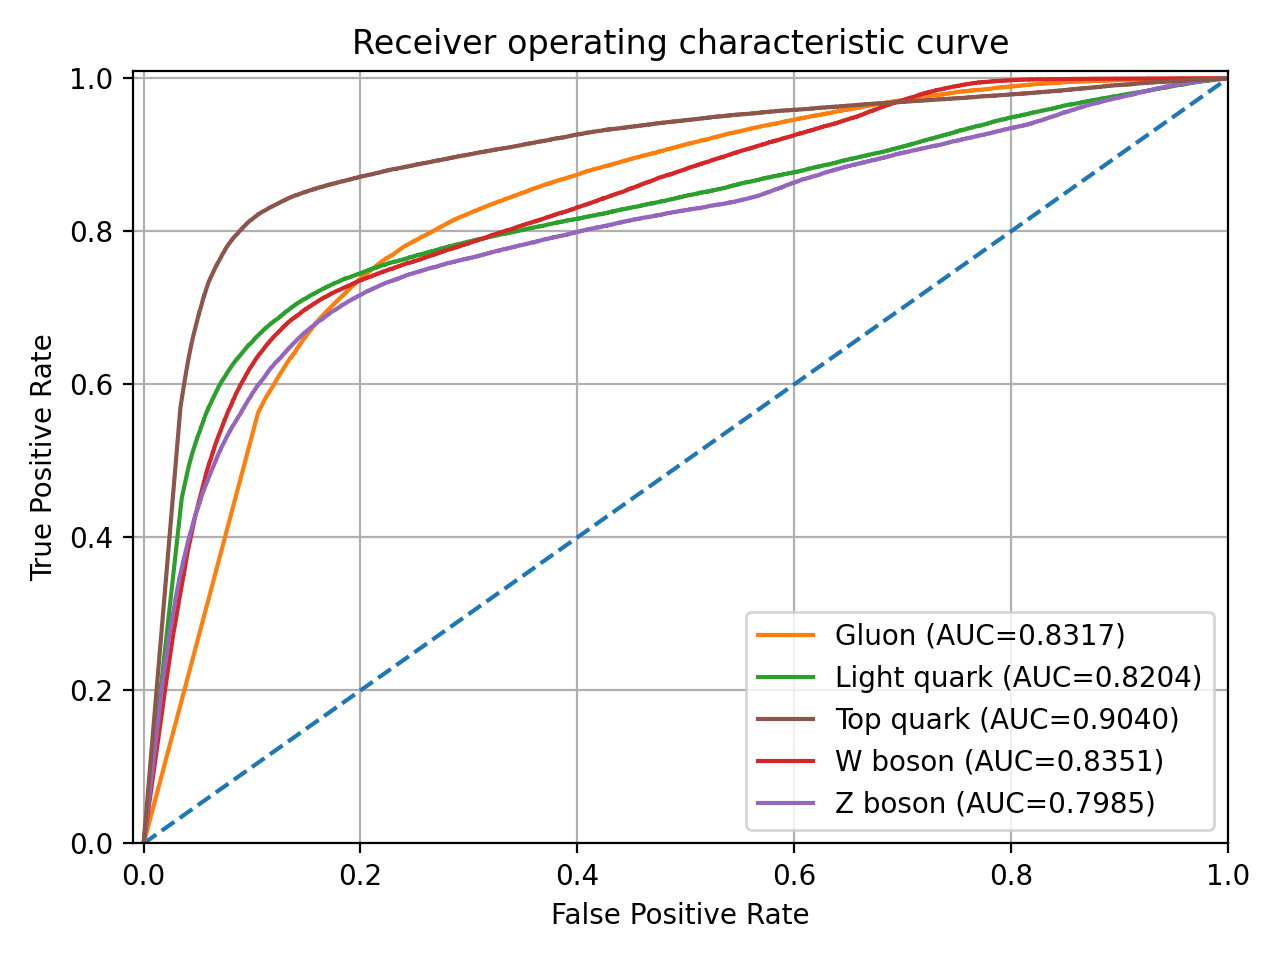
\includegraphics[trim={0cm 0cm 0cm 0cm}, width=0.6\textwidth, center]{../logs/ROC.png}
  \caption{ROC curve for TODO}
  \label{fig:ROC}
\end{figure}

\indo{Talk about grid search for accuracy-focused model as a quick and easy hyperparameter search, that was done mainly to look for simpler designs given very long synthesis, not hardcore tuning accuracy}
\indo{Give estimate of how long is the synthesis and why this is a problem}
\indo{|}
\indo{|}

\begin{figure}[hpt!]
  \centering
  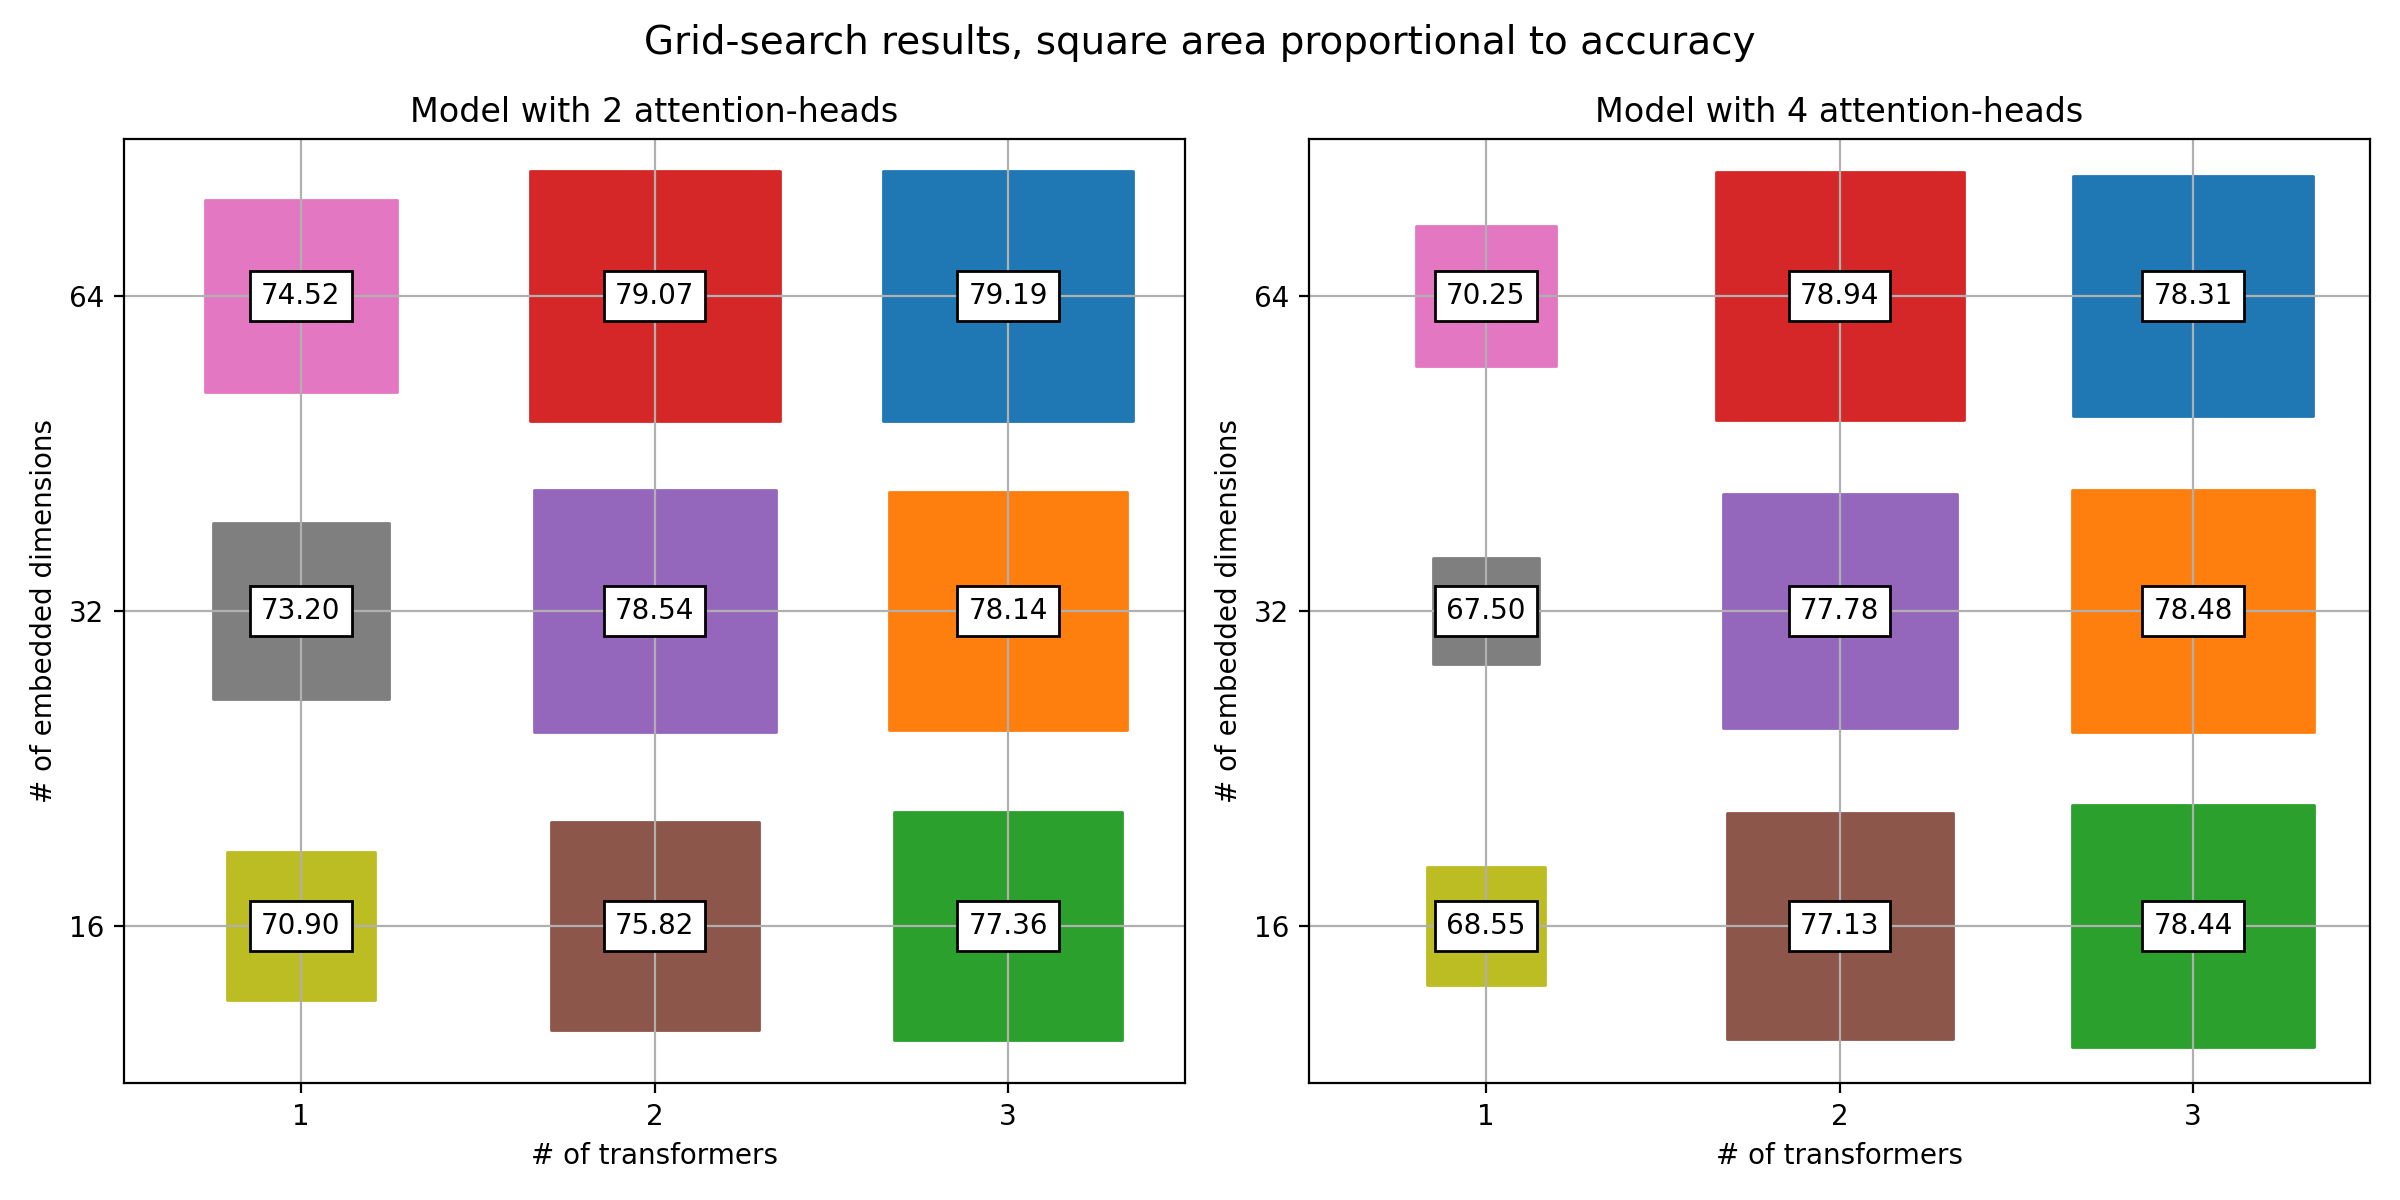
\includegraphics[trim={0cm 0cm 0cm 1cm}, clip, width=1.0\textwidth, center]{../logs/grid_search.png}
  \caption{Grid-search results - squares area proportional to accuracy.}
  \label{fig:grid-search}
\end{figure}

\indo{Ultra-low latency ROC and its meaning}
\indo{|}

\begin{figure}[hpt!]
  \centering
  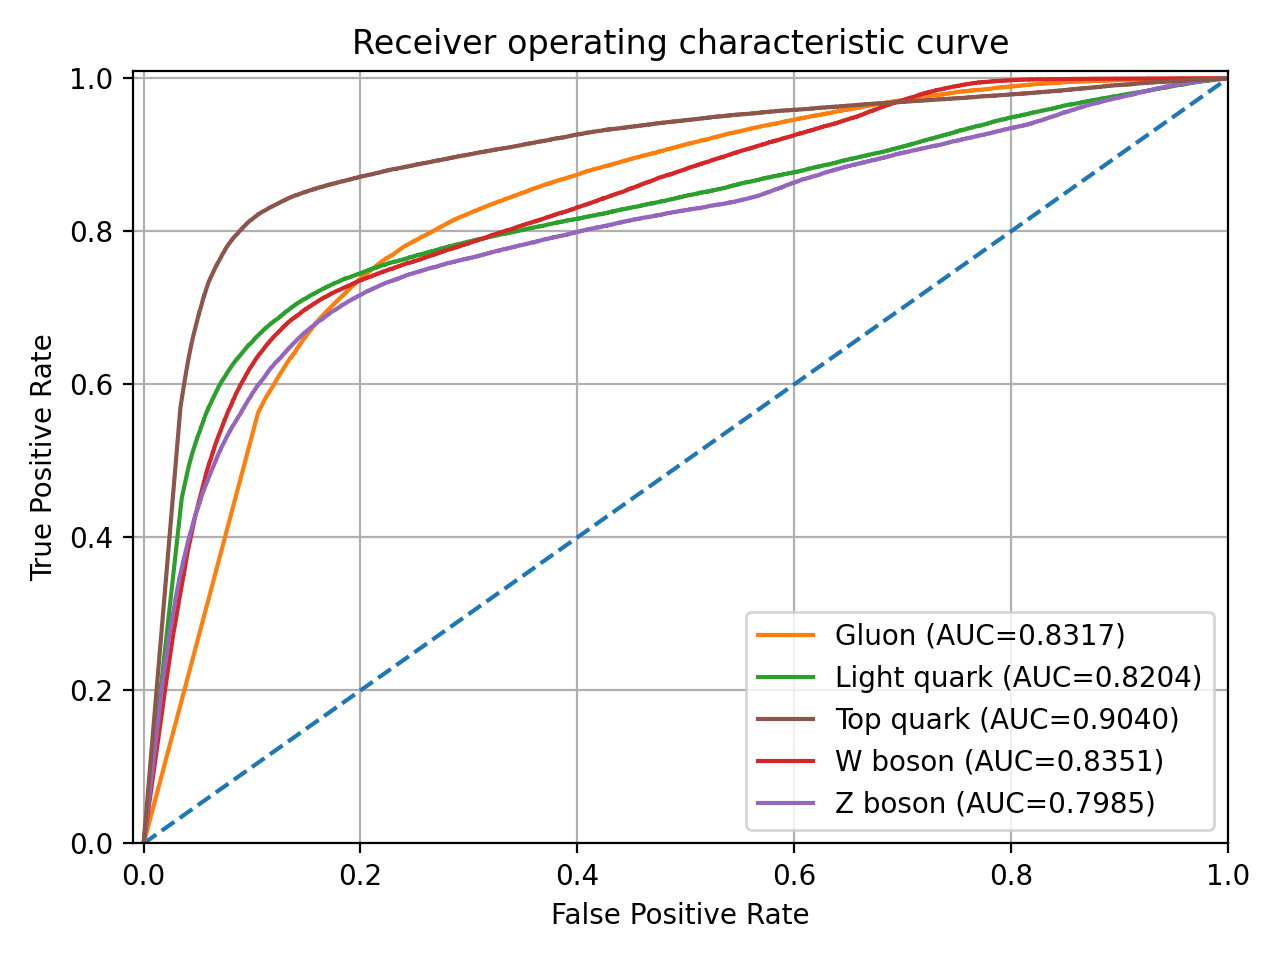
\includegraphics[trim={0cm 0cm 0cm 0cm}, width=0.6\textwidth, center]{../logs/ROC.png}
  \caption{ROC curve for TODO}
  \label{fig:ROC2}
\end{figure}

\indo{Table with AUC and accuracy}
\indo{|}
\indo{|}
\indo{|}
\indo{|}
\indo{|}

\indo{Accuracy-focused ROC and its meaning}
\indo{|}

\begin{figure}[hpt!]
  \centering
  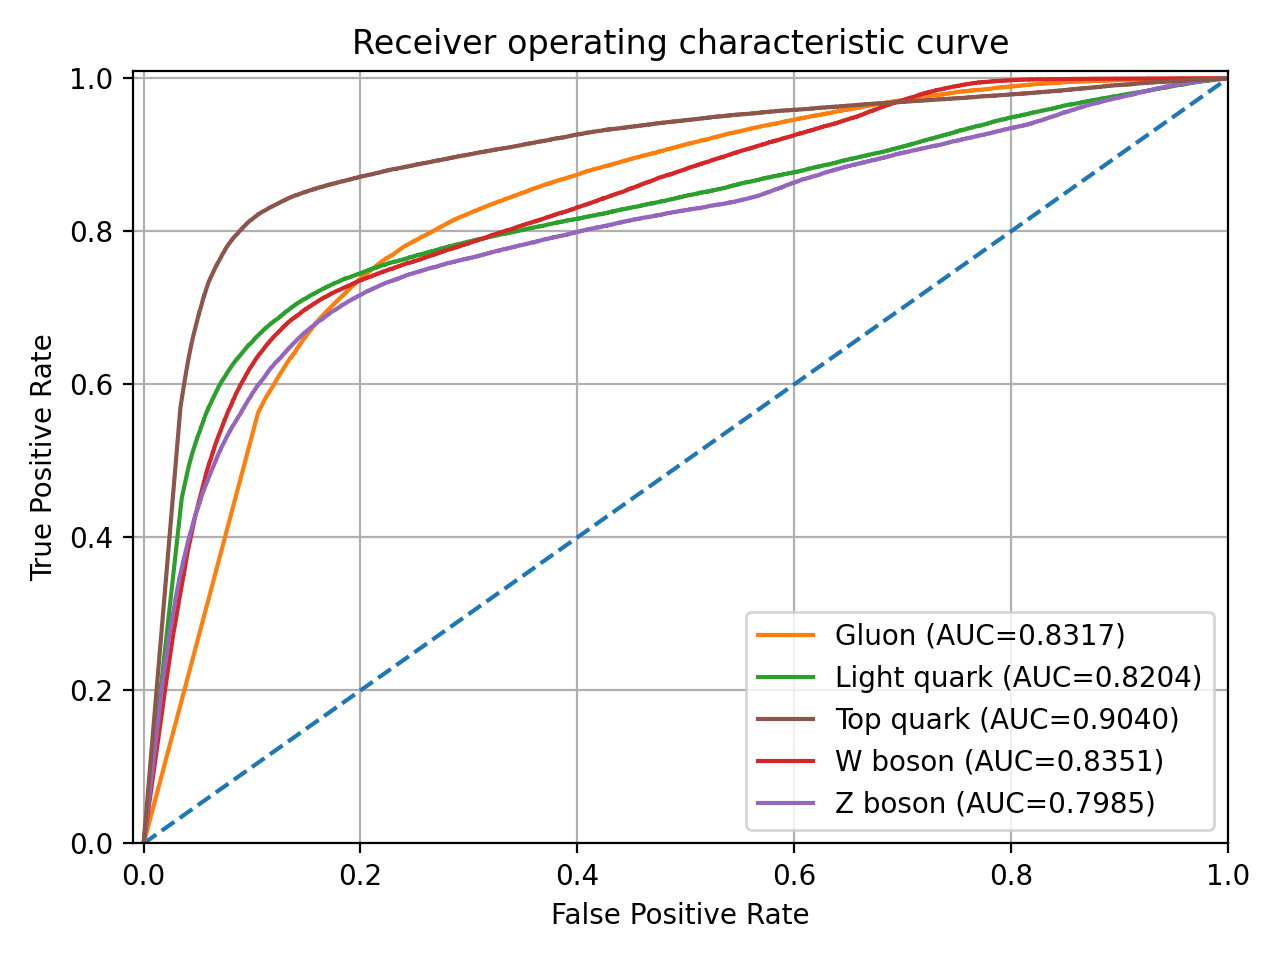
\includegraphics[trim={0cm 0cm 0cm 0cm}, width=0.6\textwidth, center]{../logs/ROC.png}
  \caption{ROC curve for TODO}
  \label{fig:ROC3}
\end{figure}

\indo{Table with AUC and accuracy}
\indo{|}
\indo{|}
\indo{|}
\indo{|}
\indo{|}


\subsection{Proposed Networks' Latency using CPUs and GPUs}

\indo{Latency on CPUs and GPUs, extend table below with accuracy-focused latency results or just create a second one}
\indo{Comment on how little difference there is between all CPUs and GPUs}
\indo{|}
\indo{|}

The detailed specifications of the machines used for measuring the inference time are listed below. The system specification is shared and includes CentOS 7.0. The first machine that hosts the GPUs has CUDA version 11.5, driver version 495.29.05.

\begin{itemize}
  \item Dual Intel Xeon Silver 4110 at 2.10GHz with 192 GB DDR4 at 2666 MT/s - GPUs host,
  \item Dual Intel Xeon X5690 at 3.47GHz with 96 GB DDR3 at 1333 MT/s,
  \item Intel Xeon E5-2620 v3 at 2.40GHz with 192 GB DDR4 at 2133 MT/s,
  \item Dual Intel Xeon Gold 6154 CPU at 3.00GHz with 768 GB DDR4 at 2666 MT/s,
\end{itemize}


\begin{table}[hpt!]
  \centering
  \caption{Comparison of simplified model's inference times with batch size of 128}
  \label{tab:inference-times}
  \bgroup
  \def\arraystretch{1.2}
  \setlength\tabcolsep{3mm}
  \begin{tabular}{c|l|cc|}
  \cline{2-4}
  \multicolumn{1}{l|}{}                               & \multicolumn{1}{c|}{\multirow{2}{*}{\textbf{Device}}}       & \multicolumn{2}{c|}{\textbf{Inference time}}                      \\ \cline{3-4} 
  \multicolumn{1}{l|}{}                               & \multicolumn{1}{c|}{}                                       & \multicolumn{1}{c|}{per batch (ms)}          & per sample ($\mu$s) \\ \hline
  \multicolumn{1}{|c|}{\multirow{4}{*}{\textbf{\begin{sideways}CPU\end{sideways}}}} & Intel Xeon Silver 4110 (Dual) & \multicolumn{1}{c|}{1.741 $\pm$ 0.027}       & 13.604 $\pm$ 0.207 \\ \cline{2-4} 
  \multicolumn{1}{|c|}{}                              & Intel Xeon X5690 (Dual)                                     & \multicolumn{1}{c|}{1.622 $\pm$ 0.026}       & 12.670 $\pm$ 0.206 \\ \cline{2-4} 
  \multicolumn{1}{|c|}{}                              & Intel Xeon E5-2620 v3                                       & \multicolumn{1}{c|}{1.325 $\pm$ 0.123}       & 10.350 $\pm$ 0.963 \\ \cline{2-4}
  \multicolumn{1}{|c|}{}                              & Intel Xeon Gold 6154 (Dual)                                 & \multicolumn{1}{c|}{1.167 $\pm$ 0.066}       & 9.112 $\pm$ 0.516  \\ \hline\hline
  \multicolumn{1}{|c|}{\multirow{3}{*}{\textbf{\begin{sideways}GPU\end{sideways}}}} & Nvidia GTX 1080 Ti            & \multicolumn{1}{c|}{1.166 $\pm$ 0.112}       & 9.111 $\pm$ 0.876  \\ \cline{2-4} 
  \multicolumn{1}{|c|}{}                              & Nvidia TITAN X                                              & \multicolumn{1}{c|}{1.154 $\pm$ 0.119}       & 9.017 $\pm$ 0.928  \\ \cline{2-4} 
  \multicolumn{1}{|c|}{}                              & Nvidia TITAN Xp                                             & \multicolumn{1}{c|}{1.062 $\pm$ 0.036}       & 8.296 $\pm$ 0.283  \\ \cline{2-4} 
  \hline
  \end{tabular}
  \egroup
\end{table}




\section{Hardware Implementation}
\indo{Small introduction}
Thanks to its high-performance, XCU250 (variant figd2104-2L-e) was chosen as the target FPGA platform.
\indo{Brief info about XCU250}

\subsection{Ultra-Low Latency Model}
\indo{Discuss hardware resources and latency}
\indo{|}
\indo{|}
\indo{|}
\indo{|}

\indo{Small table with cycles, latency, clock frequency}
\indo{|}
\indo{|}

\begin{table}[hpt!]
  \centering
  \caption{FPGA resources utilization}
  \label{tab:utilization}
  \bgroup
  \def\arraystretch{1.3}
  \setlength\tabcolsep{3mm}
  \begin{tabular}{r|c|c|c|c|}
  \cline{2-5}
  \multicolumn{1}{c|}{}                      & \textbf{BRAM 18K} & \textbf{DSP48E} & \textbf{FF} & \textbf{LUT} \\ \hline
  \multicolumn{1}{|r|}{\textbf{Total used}}       & 12                 & 4,351            & 58,942       & 298,881       \\ \hline
  \multicolumn{1}{|r|}{\textbf{Available}}   & 5,376              & 12,288           & 3,456,000     & 1,728,000      \\ \hline\hline
  \multicolumn{1}{|r|}{\textbf{Utilization}} & 0.22\%            & 35.41\%         & 1.71\%      & 17.30\%       \\ \hline
  \end{tabular}
  \egroup
\end{table}

\indo{Explain which and how the design changes affected the results below}
\indo{|}
\indo{|}
\indo{|}

\begin{figure}[hpt!]
  \centering
  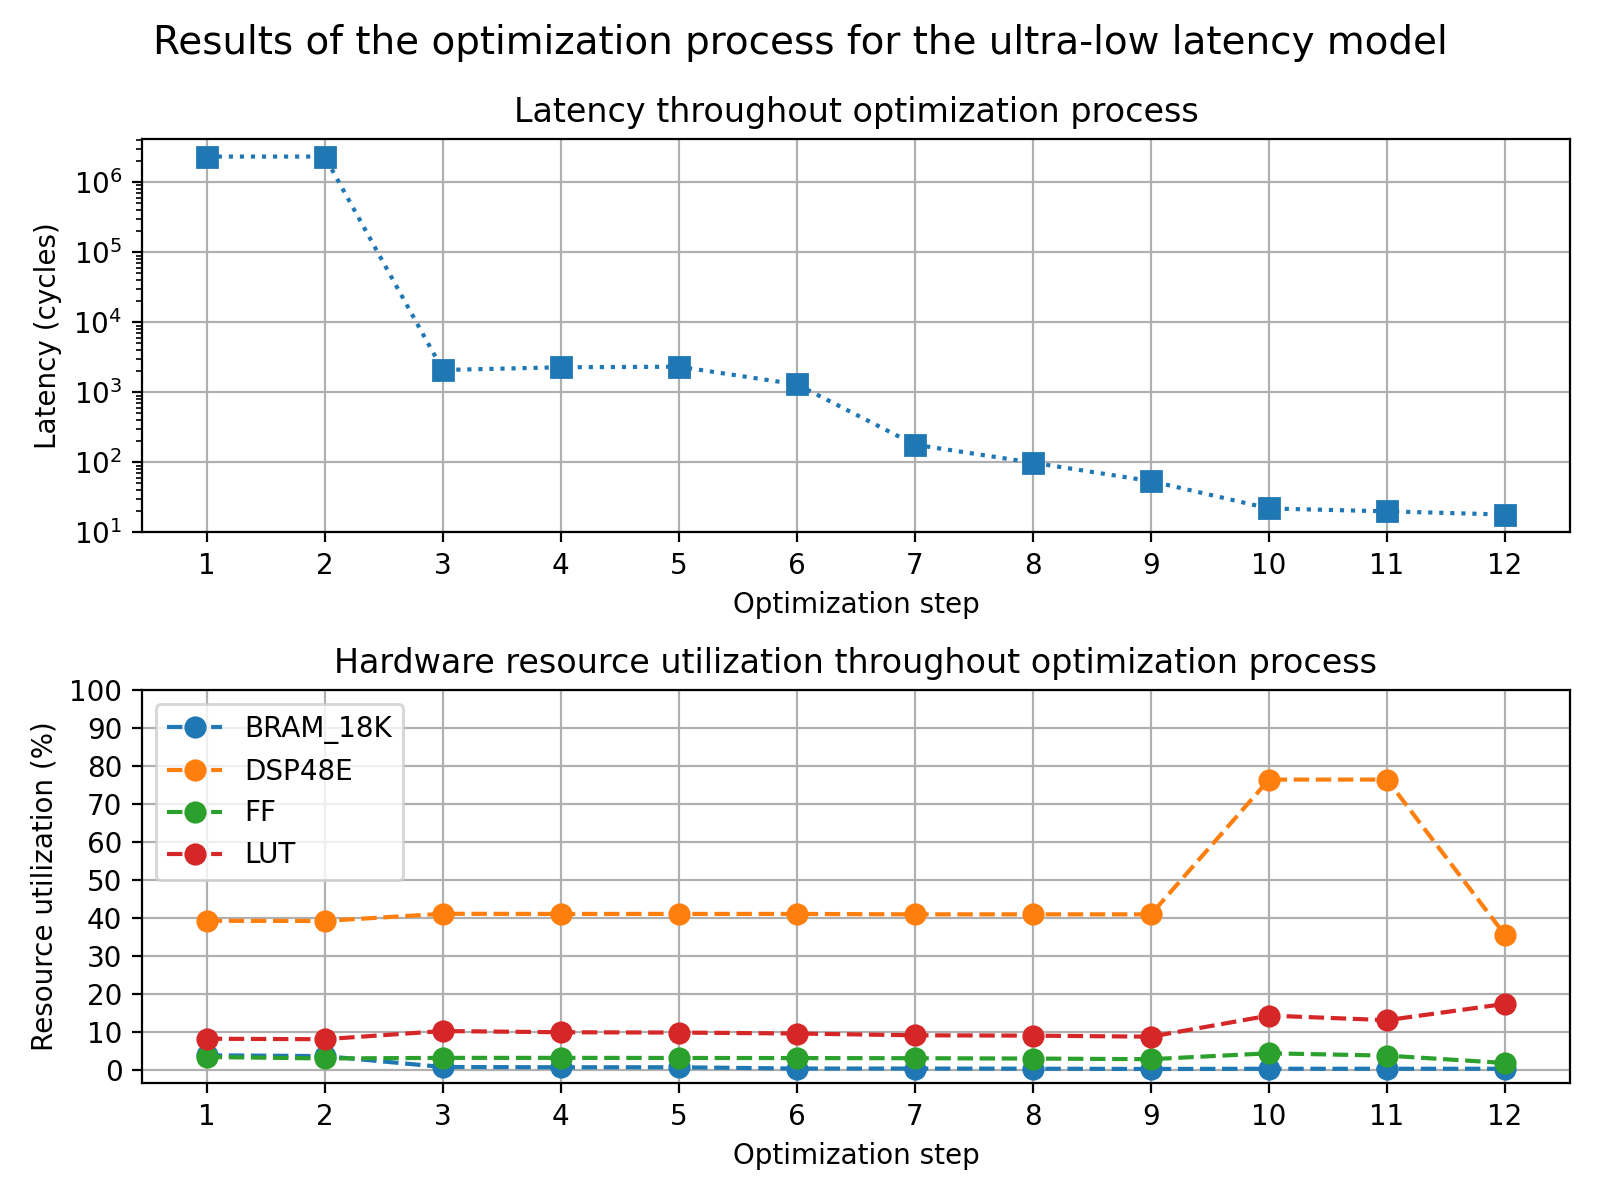
\includegraphics[trim={0cm 0cm 0cm 1cm}, clip, width=0.8\textwidth, center]{../logs/hardware_optimizations.png}
  \caption{Results of the optimization process for the ultra-low latency model.}
  \label{fig:hardware-optimizations}
\end{figure}

\indo{Talk about Pareto front and its meaning, maybe use a roofline model if it makes sense}
\indo{|}
\indo{|}
\indo{|}

\begin{figure}[hpt!]
  \centering
  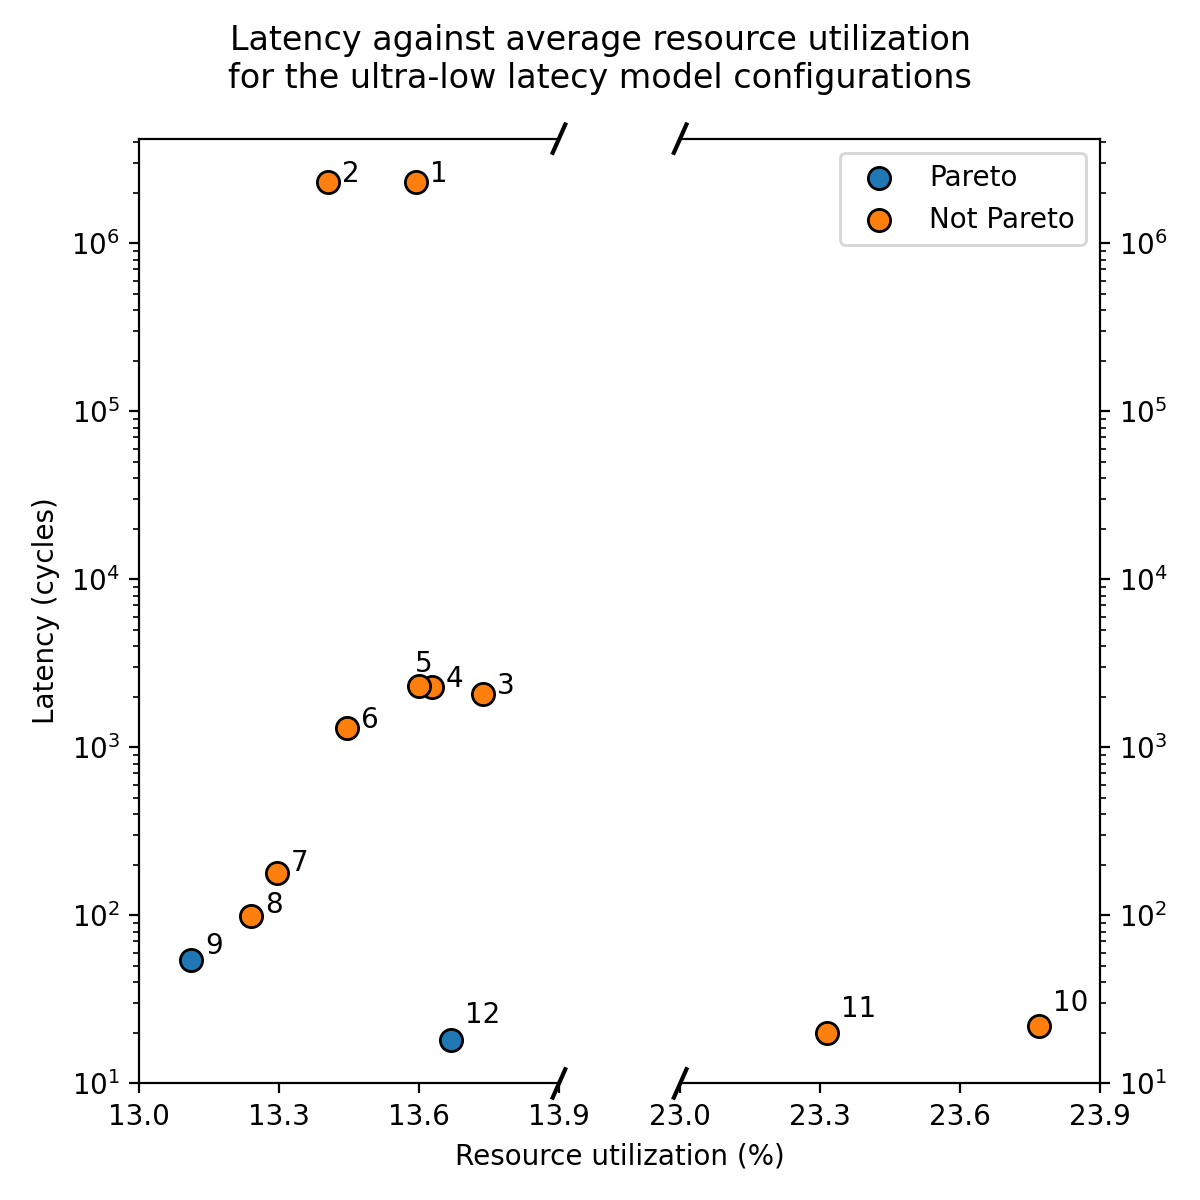
\includegraphics[trim={0cm 0cm 0cm 1.3cm}, clip, width=0.6\textwidth, center]{../logs/hardware_optimizations_pareto.png}
  \caption{Latency plotted against average resource utilization for the ultra-low latency model configurations.}
  \label{fig:hardware-optimizations-pareto}
\end{figure}


\indo{Verify analytical models for latency/resources}


\section{Quantization Results}


\subsection{Pre-Training Quantization}
\indo{Recap how this was done and talk about results}
\indo{Mention float16 doesnt learn anything (acc 20\%) as its range is too small, and we cannot consider normalizing inputs as its real time system}
\indo{Mention problems with fixed-point 32 and reason about both int and frac range being important, give examples at which point which one causes issues (likely input -> int range, after normalization -> frac range)}
\indo{Mention brevitas only gets 34\% accuracy and why this is the case and how it could be solved}
\indo{|}
\indo{|}
\indo{|}

\begin{figure}[hpt!]
  \centering
  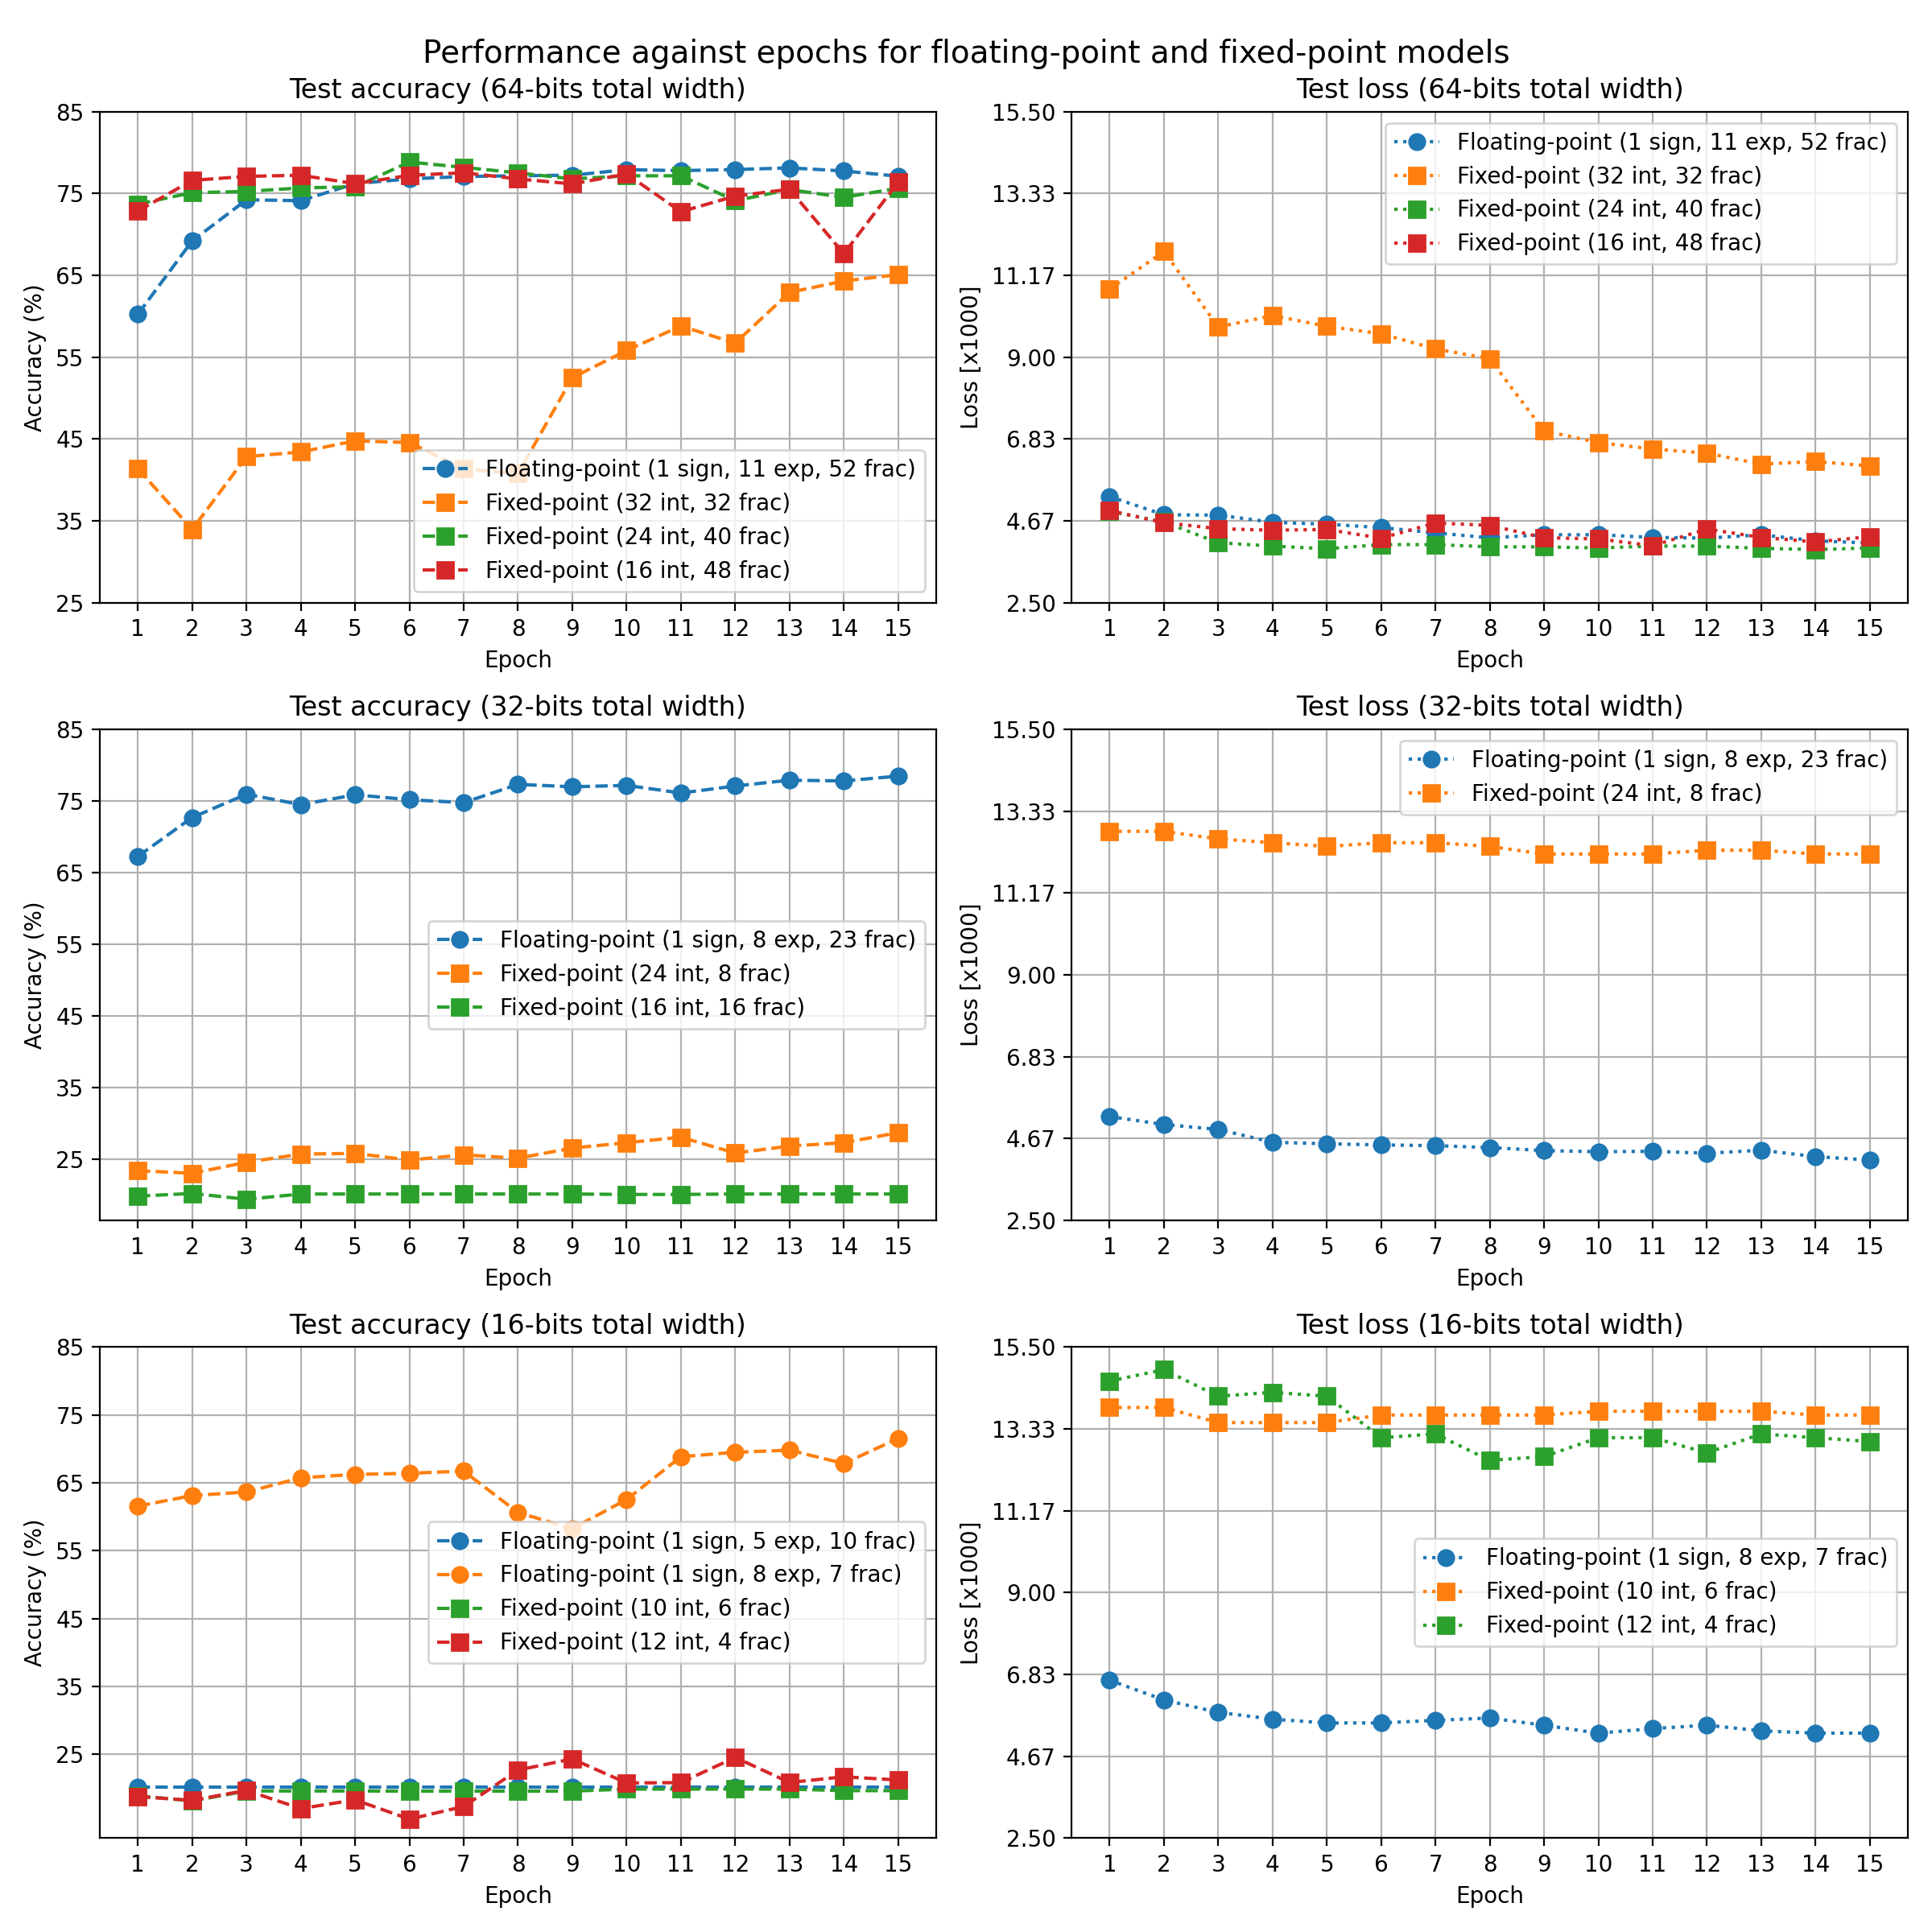
\includegraphics[trim={0cm 0cm 0cm 1.2cm}, clip, width=1.0\textwidth, center]{../logs/training_accuracy.png}
  \caption{Performance against epochs for floating-point and fixed-point models.}
  \label{fig:pre-training}
\end{figure}


\subsection{Post-Training Quantization}\label{eval:post-training-quantization}
\indo{State that the results are very promising (64\% bits reduction), how this should influence synthesis}
\indo{prove correlation with how different on average is the next bit width compared to previous vs default (34 bits etc)}
\indo{say how we dont do synthesis due to time limitations, and its mostly no problem as the widhts are linear with hardware resources aside from the situations in which a dsp can be avoided (34 vs 35 bits etc)}
\indo{Maybe talk about how correlation was verified}
\indo{starting with integer or fractional in the search didnt seem to matter in the limited tests}
\indo{Discuss the used parameters (ratio of positive and negative tolerance etc.) and how they affect the results}
\indo{|}
\indo{|}

\begin{figure}[hpt!]
  \centering
  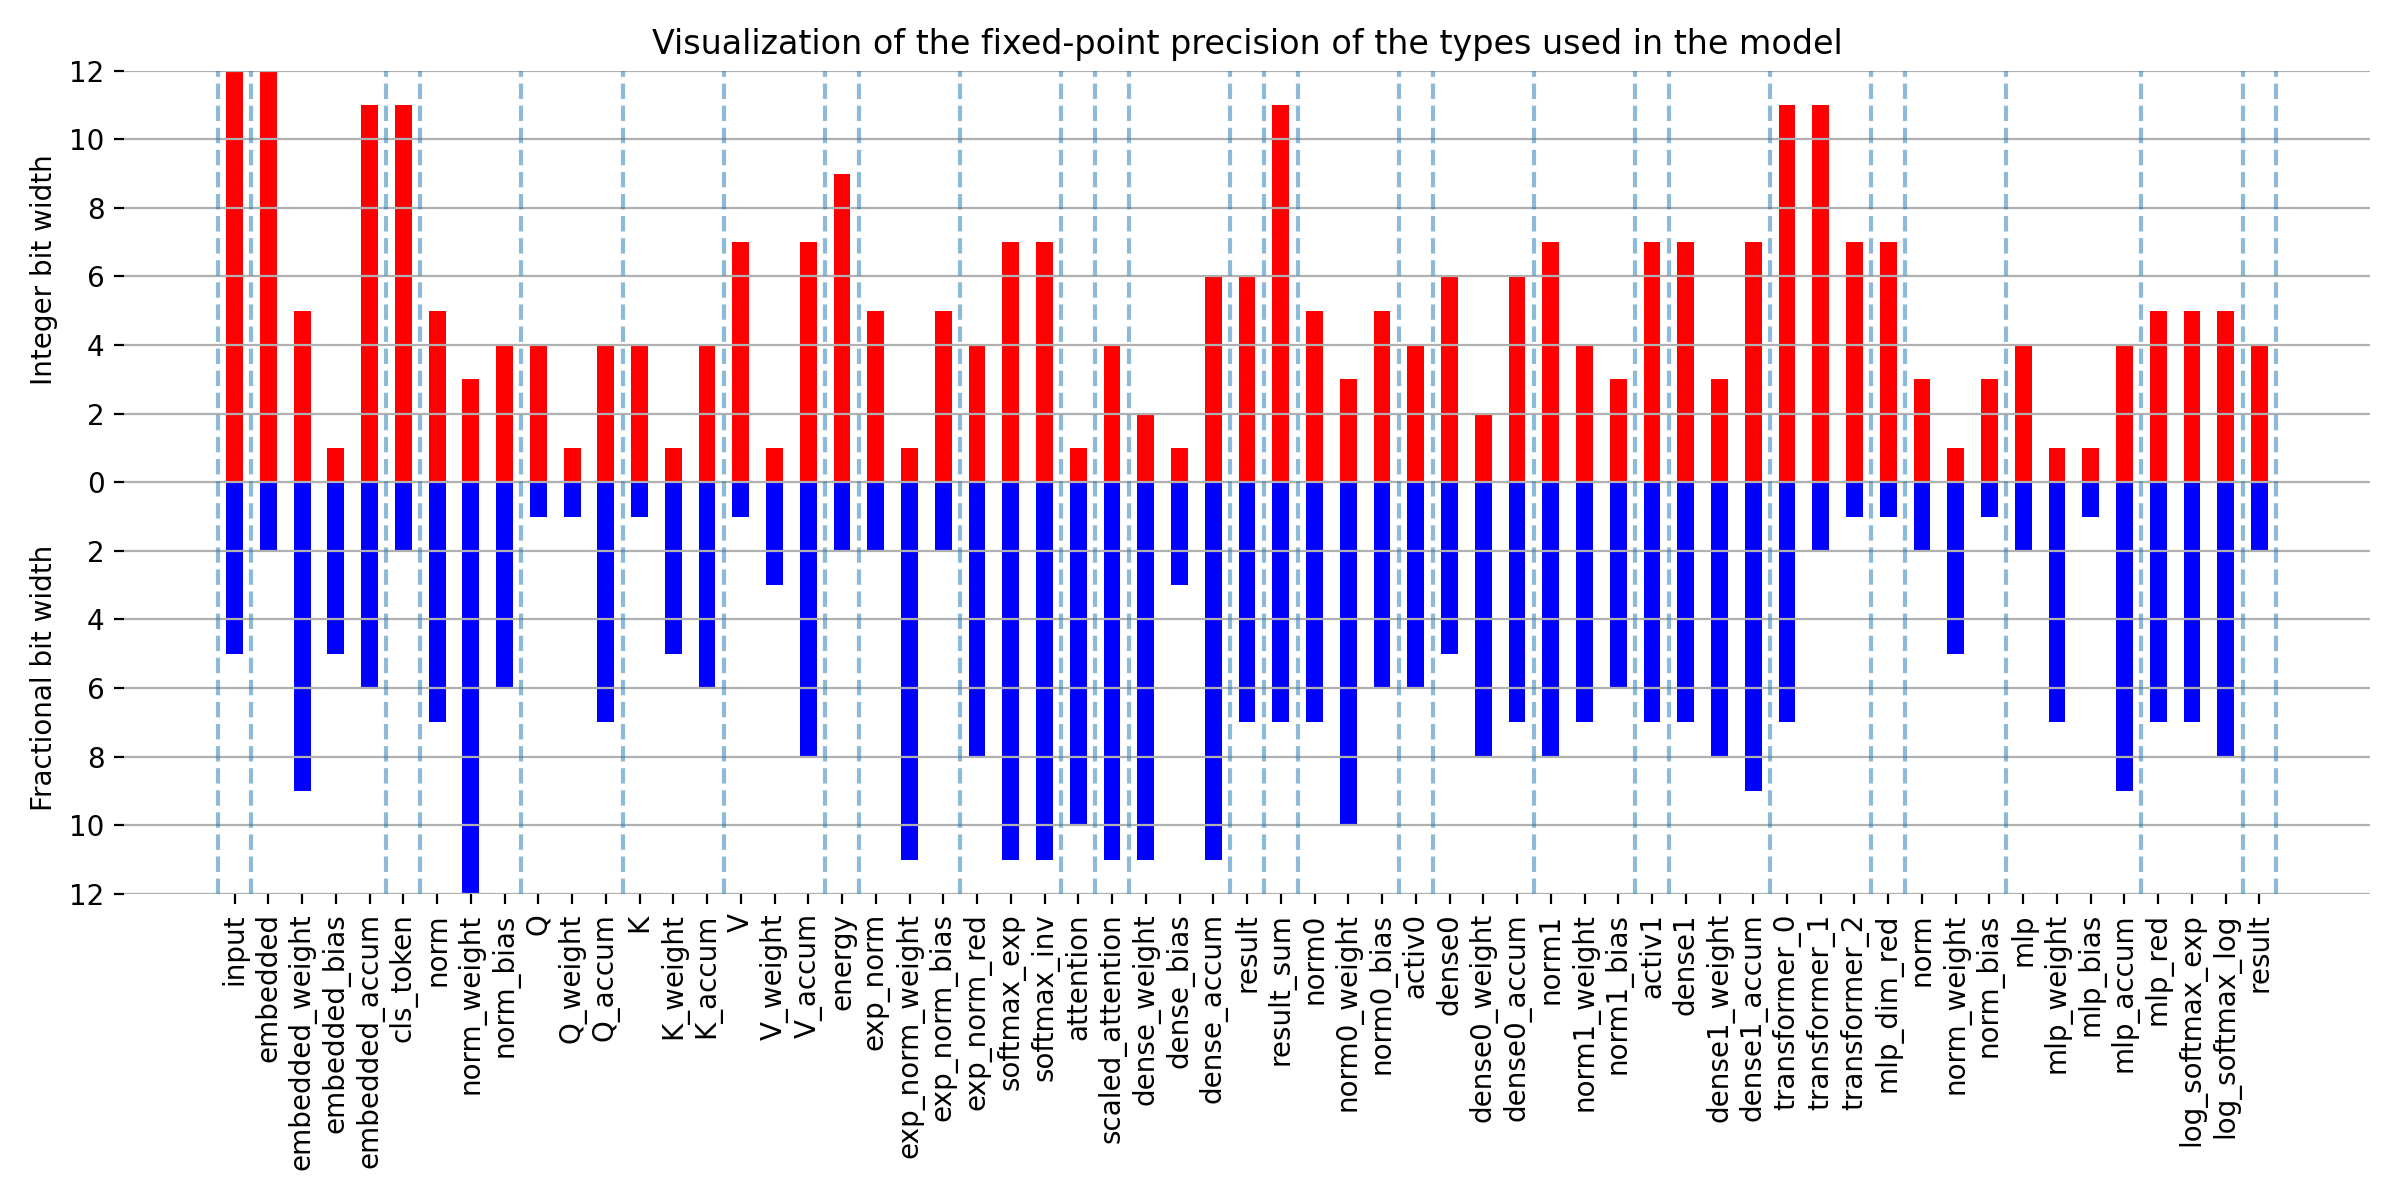
\includegraphics[trim={0cm 0cm 1cm 7.8mm}, clip, width=1.0\textwidth, center]{../logs/bit_width_visualization.png}
  \caption{Visualization of the fixed-point precision of the types used in the accuracy-focused model.}
  \label{fig:post-training-bit-widths}
\end{figure}
